\section{Ejecucion del juego}

\subsection{Configuración Inicial}
El juego comienza con la bienvenida y la solicitud para que los Jugadores 1 y 2 elijan un reino diferente. En este ejemplo, el Jugador 2 selecciona el reino de Francia y la posición 4 en el tablero.

\begin{lstlisting}[language=plaintext]
Jugador 1 y 2, escojan un reino(diferentes):
(1)Inglaterra
(2)Francia
(3)Sacro Imperio
(4)Castilla-Aragon
(5)Moros
2
4
\end{lstlisting}

\subsection{Estado Inicial del Tablero}
Se presenta el tablero de soldados con las posiciones iniciales de las unidades.

\begin{lstlisting}[language=plaintext]
Tablero de soldados
 _____________________________________________________________________
|______|______|______|______|______|X-C11 |______|______|______|______|
|______|______|______|______|______|X-EC14|______|Z-CF15|______|______|
|______|______|______|______|______|______|______|______|______|______|
|______|______|______|______|______|______|______|______|______|______|
|______|______|______|______|______|______|______|Z-C10 |______|______|
|X-C11 |______|______|______|X-L6  |______|______|______|______|______|
|______|______|______|______|______|______|______|______|______|______|
|Z-L6  |______|______|______|______|______|______|______|______|______|
|______|______|______|______|______|______|______|______|______|X-E8  |
|______|______|______|______|______|______|X-L5  |______|______|______|
\end{lstlisting}

\subsection{Información Detallada de los Soldados}
A continuación, se presentan los datos detallados de cada soldado en los ejércitos Z y X.

\begin{lstlisting}[language=plaintext]
----------Datos de los soldados Z0------------
CaballeroZ0          (Z-C10 ) | Vida:10 | Fila:4 | Columna:7 | Atq:13 | Def:7
LanceroZ0            (Z-L6  ) | Vida:6  | Fila:7 | Columna:0 | Atq:5  | Def:10
CaballeroFrancoZ0    (Z-CF15) | Vida:15 | Fila:1 | Columna:7 | Atq:13 | Def:7
\end{lstlisting}

\begin{lstlisting}[language=plaintext]
----------Datos de los soldados X0------------
EspadachinX0         (X-E8  ) | Vida:8  | Fila:8 | Columna:9 | Atq:10 | Def:8
CaballeroX0          (X-C11 ) | Vida:11 | Fila:0 | Columna:5 | Atq:13 | Def:7
CaballeroX1          (X-C11 ) | Vida:11 | Fila:5 | Columna:0 | Atq:13 | Def:7
LanceroX0            (X-L6  ) | Vida:6  | Fila:5 | Columna:4 | Atq:5  | Def:10
LanceroX1            (X-L5  ) | Vida:5  | Fila:9 | Columna:6 | Atq:5  | Def:10
EspadachinConquistaX0(X-EC14) | Vida:14 | Fila:1 | Columna:5 | Atq:10 | Def:8
\end{lstlisting}

\subsection{Ejército Nro1 (Z) - Estadísticas y Ranking}
Se presentan las estadísticas del Ejército Nro1 (Z), incluyendo el soldado con mayor nivel de vida y el ranking de poder.

\begin{lstlisting}[language=plaintext]
-----Ejercito Nro1(Z)----
Soldado con mayor nivel de vida:
CaballeroFrancoZ0 | Vida:15 | Fila:1 | Columna:7 | Atq:13 | Def:7
Promedio de nivel de vida: 10.33
\end{lstlisting}

\begin{lstlisting}[language=plaintext]
RANKING DE PODER
----------Datos de los soldados Z0------------
CaballeroFrancoZ0    (Z-CF15) | Vida:15 | Fila:1 | Columna:7 | Atq:13 | Def:7
CaballeroZ0          (Z-C10 ) | Vida:10 | Fila:4 | Columna:7 | Atq:13 | Def:7
LanceroZ0            (Z-L6  ) | Vida:6  | Fila:7 | Columna:0 | Atq:5  | Def:10
\end{lstlisting}

\subsection{Ejército Nro2 (X) - Estadísticas y Ranking}
Se presentan las estadísticas del Ejército Nro2 (X), incluyendo el soldado con mayor nivel de vida y el ranking de poder.

\begin{lstlisting}[language=plaintext]
-----Ejercito Nro2(X)----
Soldado con mayor nivel de vida:
EspadachinConquistaX0 | Vida:14 | Fila:1 | Columna:5 | Atq:10 | Def:8
Promedio de nivel de vida: 9.17
\end{lstlisting}

\begin{lstlisting}[language=plaintext]
RANKING DE PODER
----------Datos de los soldados X0------------
EspadachinConquistaX0(X-EC14) | Vida:14 | Fila:1 | Columna:5 | Atq:10 | Def:8
CaballeroX0          (X-C11 ) | Vida:11 | Fila:0 | Columna:5 | Atq:13 | Def:7
CaballeroX1          (X-C11 ) | Vida:11 | Fila:5 | Columna:0 | Atq:13 | Def:7
EspadachinX0         (X-E8  ) | Vida:8  | Fila:8 | Columna:9 | Atq:10 | Def:8
LanceroX0            (X-L6  ) |
 Vida:6  | Fila:5 | Columna:4 | Atq:5  | Def:10
LanceroX1            (X-L5  ) | Vida:5  | Fila:9 | Columna:6 | Atq:5  | Def:10
\end{lstlisting}

\subsection{Resumen del Juego}
Se proporciona un resumen de los ejércitos creados y se evalúa el ejército con mayor probabilidad de victoria.

\begin{lstlisting}[language=plaintext]
Ejercito1: Francia
Cantidad total de soldados creados: 3
Espadachines: 0
Arqueros: 0
Caballeros: 2
Lanceros: 1
\end{lstlisting}

\begin{lstlisting}[language=plaintext]
Ejercito1: Castilla-Aragon
Cantidad total de soldados creados: 6
Espadachines: 2
Arqueros: 0
Caballeros: 2
Lanceros: 2
\end{lstlisting}

\begin{lstlisting}[language=plaintext]
---Metrica: Ejercito con mas soldados---
Ejercito 1: Francia   : 31   36.05% de probabilidad de victoria
Ejercito 2: Castilla-Aragon: 55   63.95% de probabilidad de victoria

El ganador es el . Ya que al generar los
porcentajes de probabilidad de victoria basada en los niveles de
vida de sus soldados y aplicando un experimento aleatorio salió
vencedor. (Aleatorio generado: 56.72%)
Quieres seguir jugando?(true/false)
\end{lstlisting}

El juego "SHOOTGAME" se ejecutó exitosamente, proporcionando información detallada sobre la configuración inicial, el estado de los soldados y el análisis estratégico de los ejércitos. La probabilidad de victoria se determina según la vida de los soldados, y en este caso, el ejército Castilla-Aragon se coronó como el ganador.


\subsection{Representación gráfica}
\begin{itemize}
  \item La representación visual está hecha con Java Swing y es la siguiente: 
\end{itemize}

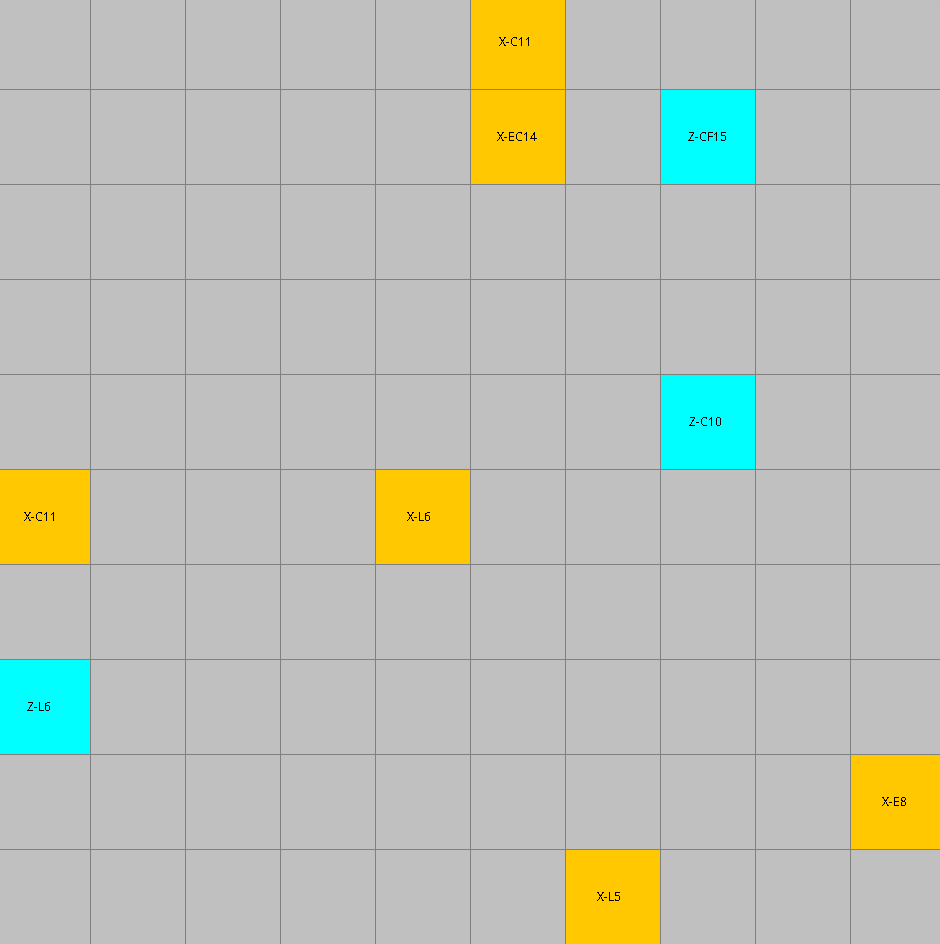
\includegraphics[width=0.50\textwidth]{img/exec.jpg}
